\documentclass{beamer}
\usepackage{amsmath}
\usepackage{icomma}
\usepackage[utf8]{inputenc}
\usepackage[T1]{fontenc}
\usepackage{polski}
\usepackage[polish]{babel}
\usepackage{hyperref}
\usepackage{float}
\usepackage{textcomp}
\usetheme{Darmstadt}
\usecolortheme{rose}

% Naprawa nazw z angielskiego
\def\figureautorefname{Rysunek}

%Strona streszczenia
\newenvironment{abstractpage}
  {\cleardoublepage\vspace*{\fill}\thispagestyle{empty}}
  {\vfill\cleardoublepage}
  
%Samo streszczenie
\newenvironment{abstractsection}[1]
  {\bigskip\selectlanguage{#1}%
   \begin{center}\bfseries\abstractname\end{center}}
  {\par\bigskip}

%Ładne ułamki w jednostkach fizycznych
\sisetup{per-mode=symbol}%

\beamertemplatenavigationsymbolsempty
\setbeamertemplate{footline}[frame number]

\begin{document}
	\section{Wprowadzenie}
	\begin{frame}
		\title[Omnivelma]{Symulacja dookólnej bazy mobilnej}
		\author{Radosław Świątkiewicz}
		\date{\today}
		\institute{Promotor: dr hab. inż. Wojciech Szynkiewicz \\ \footnotesize Instytut Automatyki i Informatyki Stosowanej \\ Wydział Elektroniki i Technik Informacyjnych \\ Politechnika Warszawska}
		\titlepage
	\end{frame}
	\begin{frame}
		\frametitle{Spis treści}
		\tableofcontents[currentsection]
	\end{frame}
	
	\section{Problem}
	\begin{frame}
		\frametitle{Platforma mobilna}
		\begin{columns}[c]
			\column{0.5\textwidth}
			\centering
			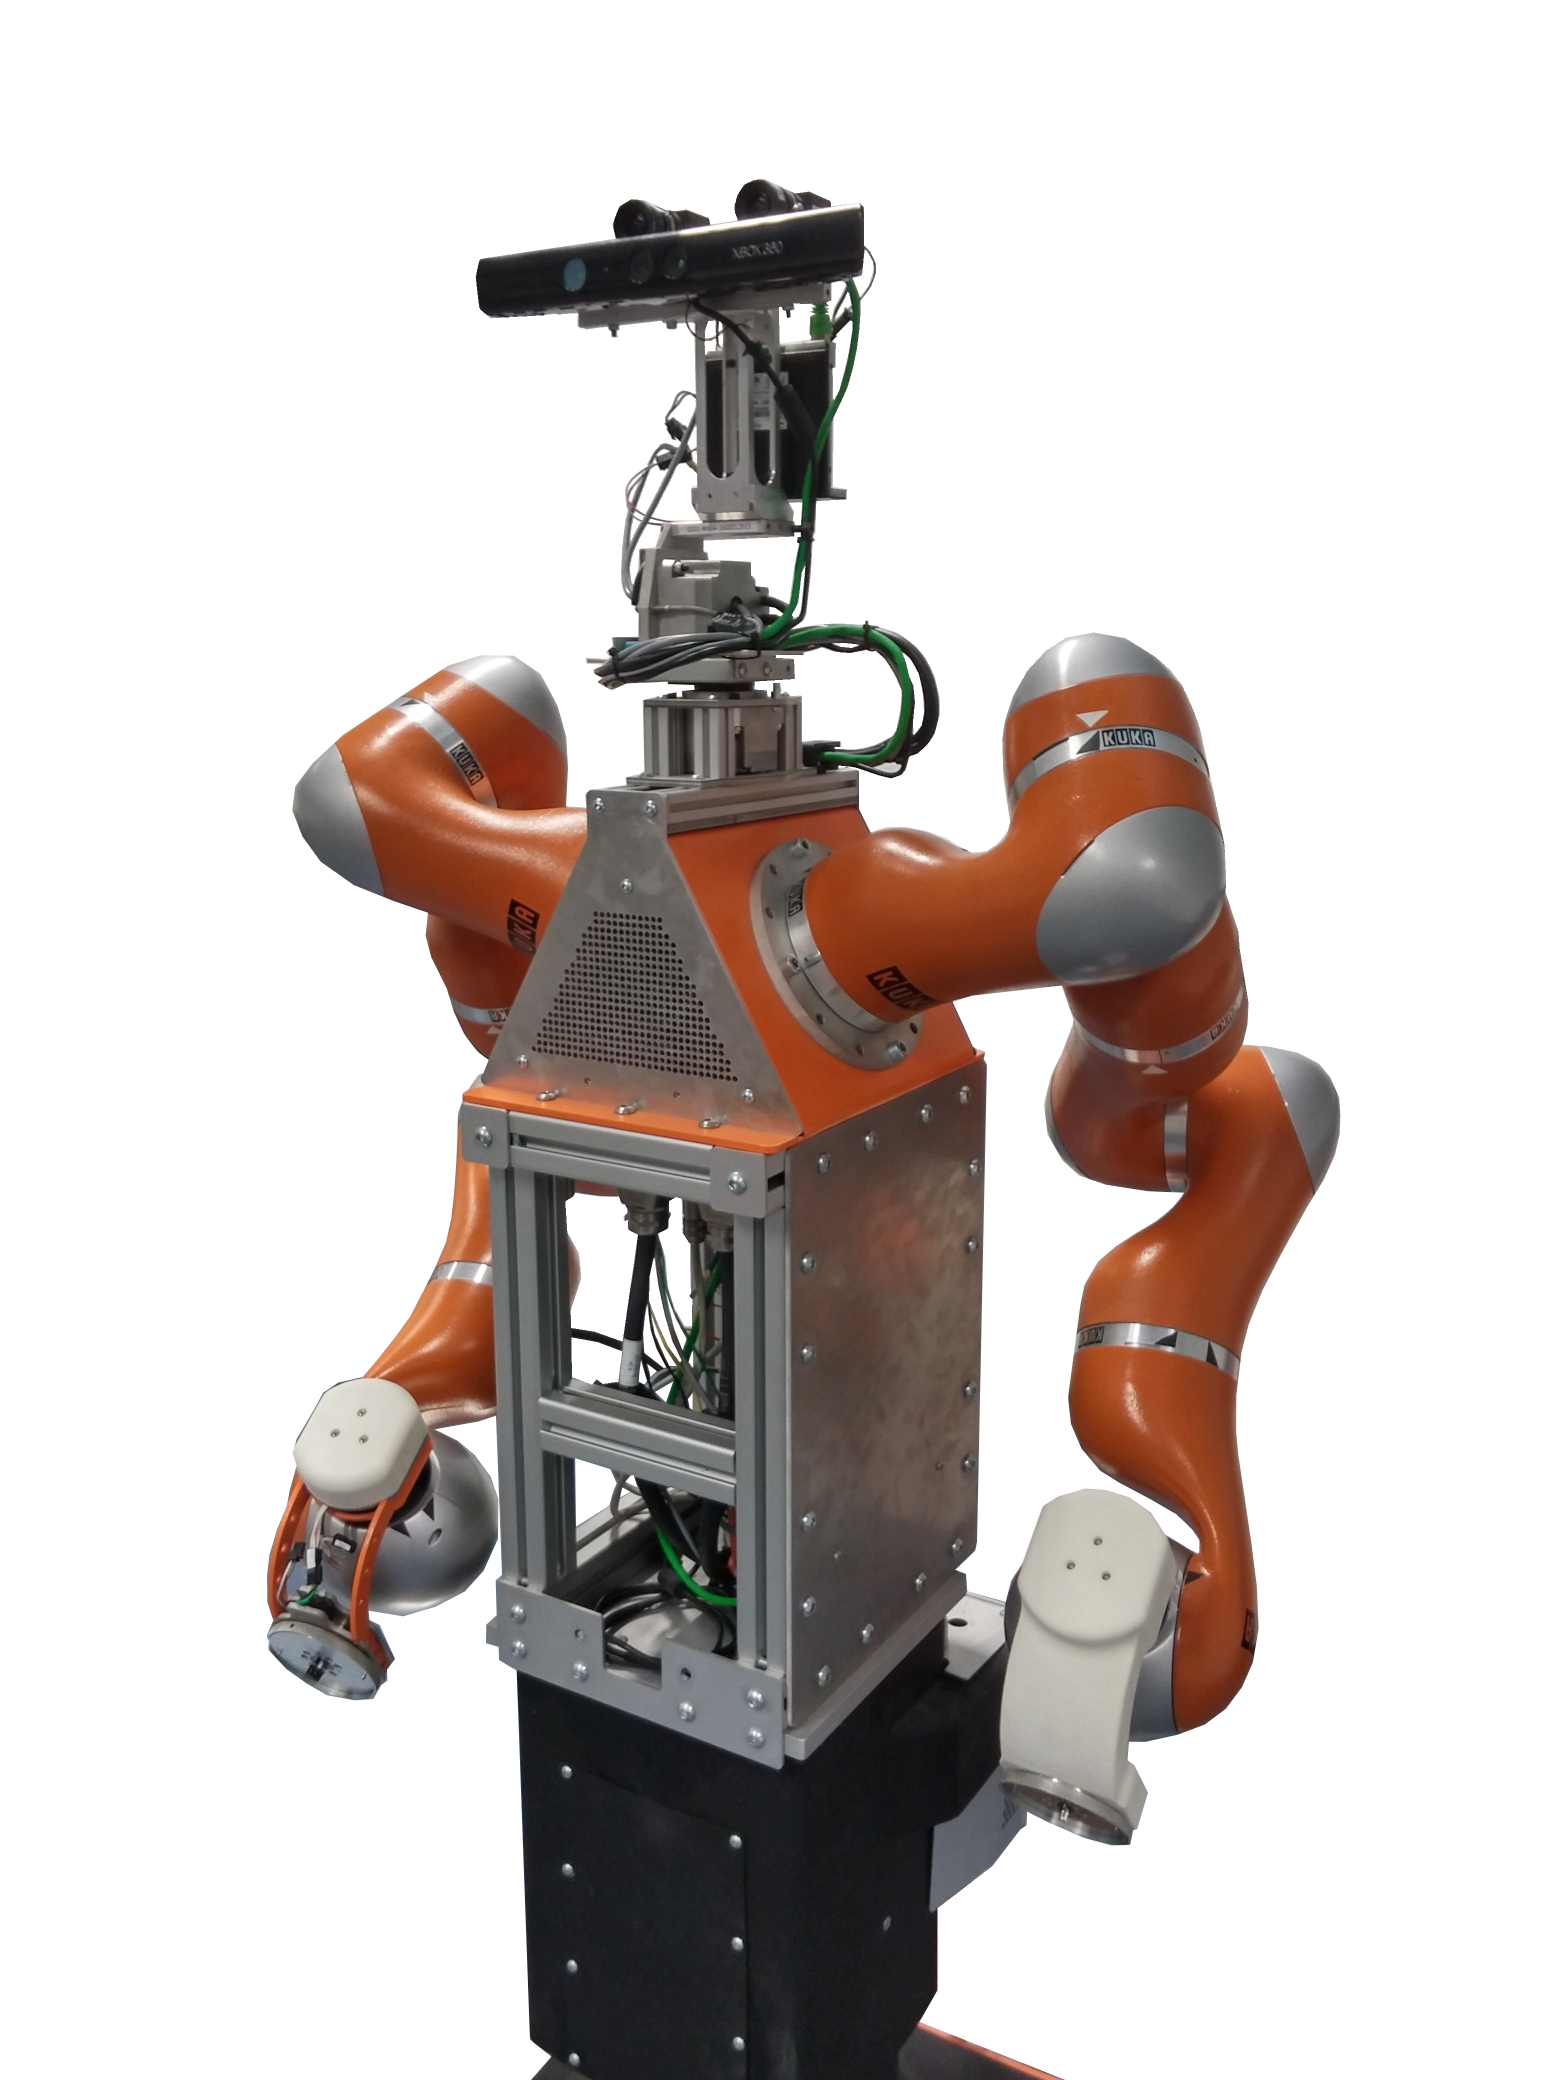
\includegraphics[width=0.8\textwidth]{graphics/velma.png} \\
			Robot manipulacyjny Velma
			\column{0.5\textwidth}
			\centering
			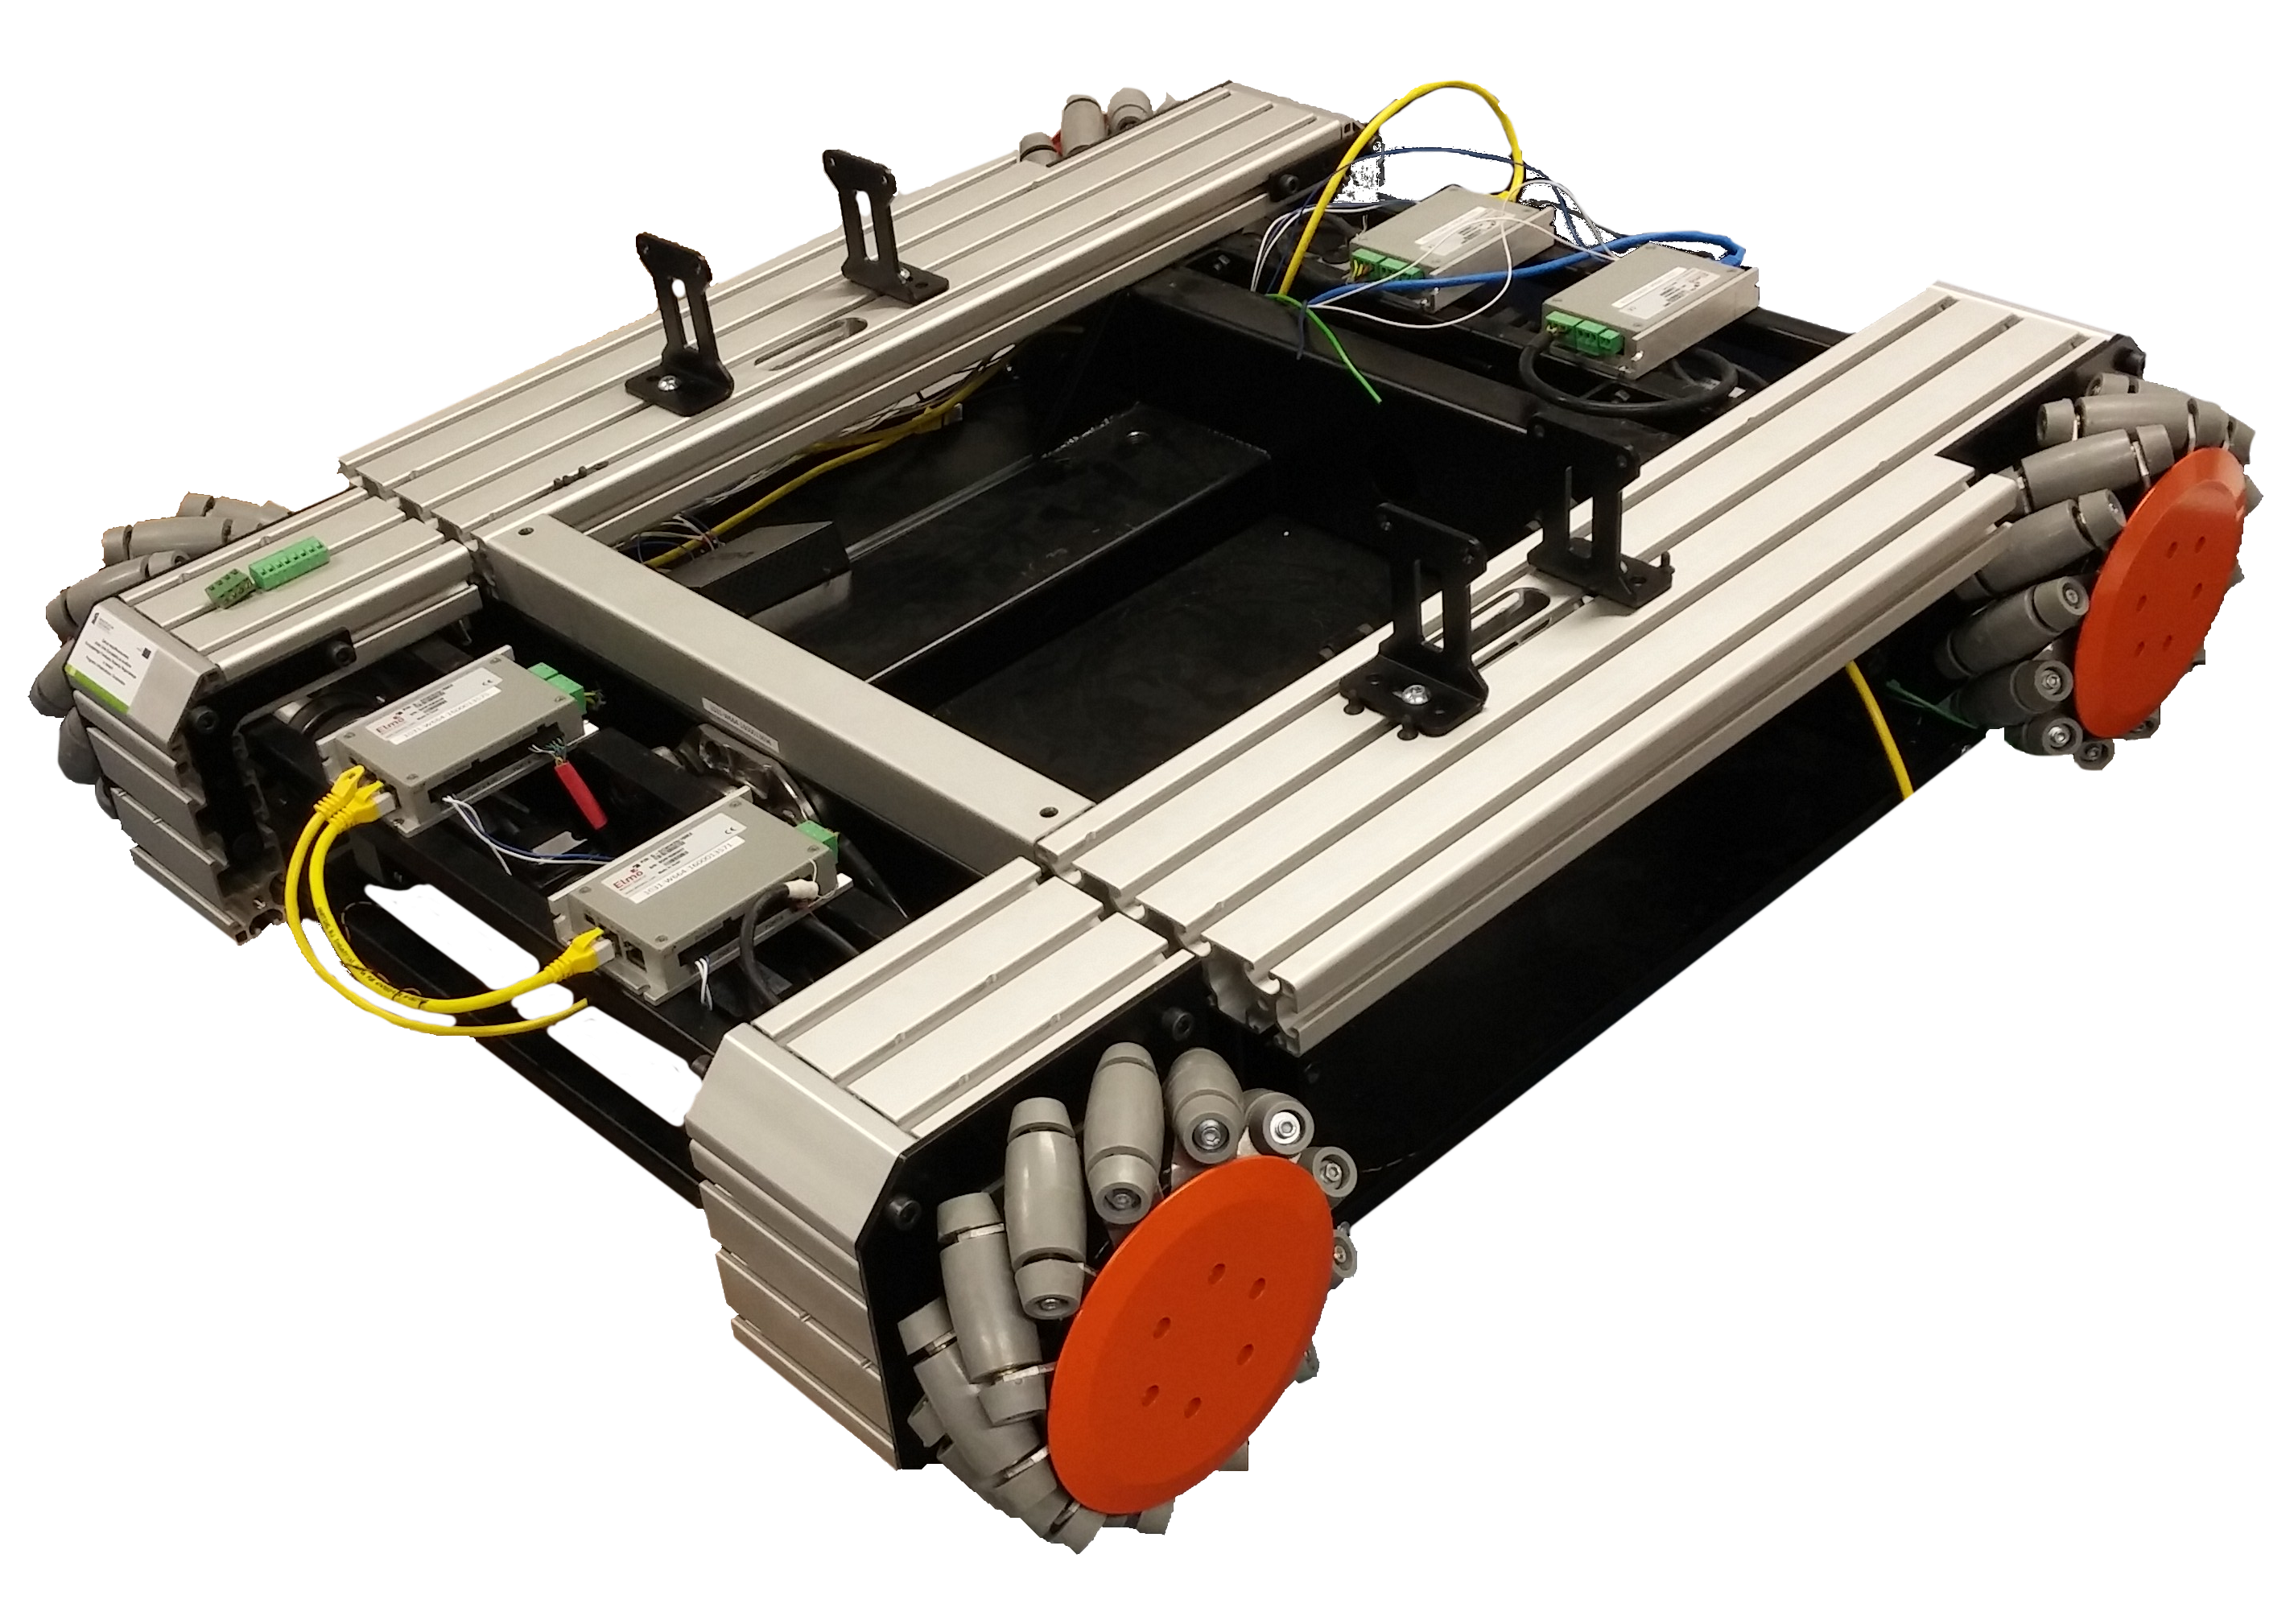
\includegraphics[width=\textwidth]{graphics/omnivelma.png} \\
			Platforma na kołach Mecanum
		\end{columns}
	\end{frame}
	\begin{frame}
		\frametitle{Cel projektu --- opracowanie modelu symulacyjnego platformy}
		Do czego przydatny jest model:
		\begin{itemize}
			\item Pozwala bezpiecznie testować nowe oprogramowanie.
			\item Przyspiesza implementację i testowanie.
			\item Ułatwia przeprowadzanie skomplikowanych i niebezpiecznych dla robota testów.
			\item Daje możliwość implementacji czujników niezamontowanych w urządzeniu.
		\end{itemize}
		Wymagania:
		\begin{itemize}
			\item Model reaguje na momenty siły i tarcie w sposób zbliżony do robota.
			\item Przyjmuje taką samą postać sygnałów sterujących.
			\item Generuje dane z czujników wirtualnych, zbliżone do rzeczywistych.
		\end{itemize}
	\end{frame}
	\begin{frame}
		\frametitle{Założenia}
		\begin{itemize}
			\item Symulacja kół musi być przybliżona ze względu na ograniczoną moc obliczeniową komputera.
			\item Robot i model poruszają się tylko po płaszczyźnie.
			\item Odwzorowujemy kinematykę, dynamikę i tarcie.
			\item Mogą występować poślizgi kół.
			\item Symulacja obarczona jest naturalnym błędem liczb zmiennoprzecinkowych.
		\end{itemize}
	\end{frame}

	\section{Platforma}
	\begin{frame}
		\frametitle{Budowa}
		\centering
		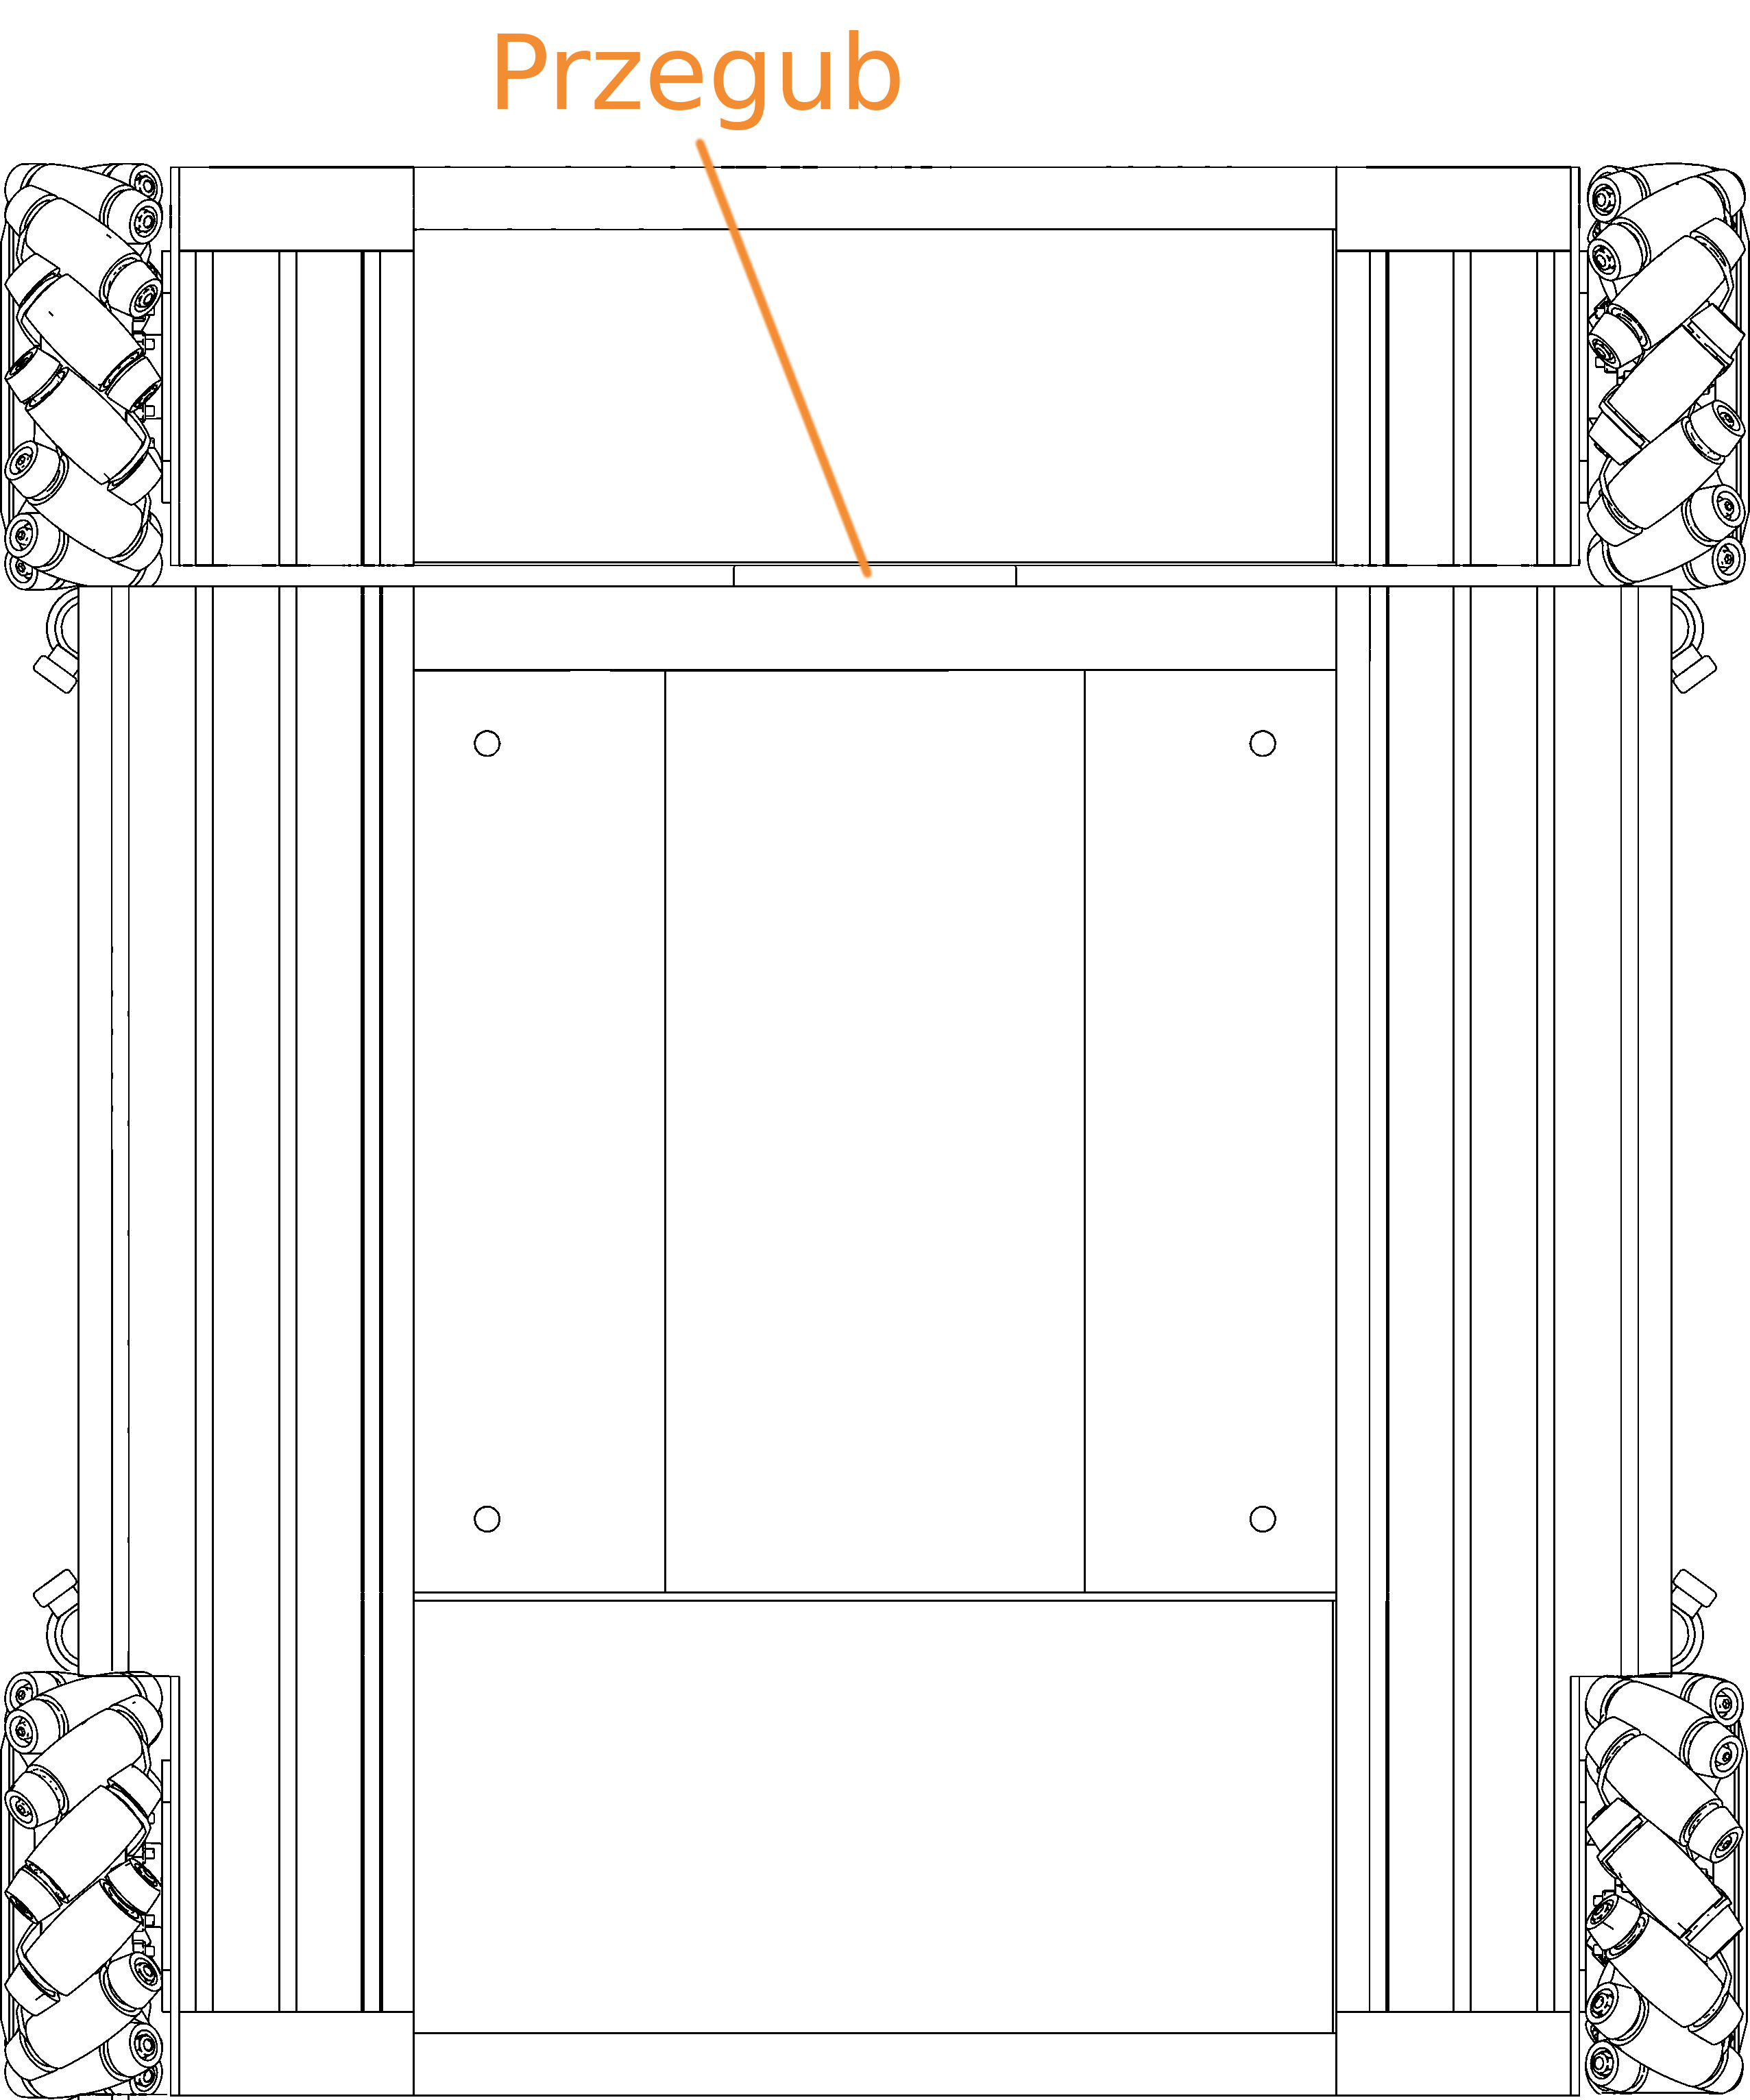
\includegraphics[width=0.4\textwidth]{graphics/base_top.png}
		\begin{itemize}
			\item Przegub zawiasowy łączy dwie części platformy.
			\item Koła ustawione są w kształt litery \emph{X}.
			\item Oś rolki aktualnie znajdującej się u góry koła jest prostopadła do osi rolki kolidującej z podłożem.
		\end{itemize}
	\end{frame}

	\begin{frame}
		\frametitle{Koła Szwedzkie (Mecanum)}
		\centering
		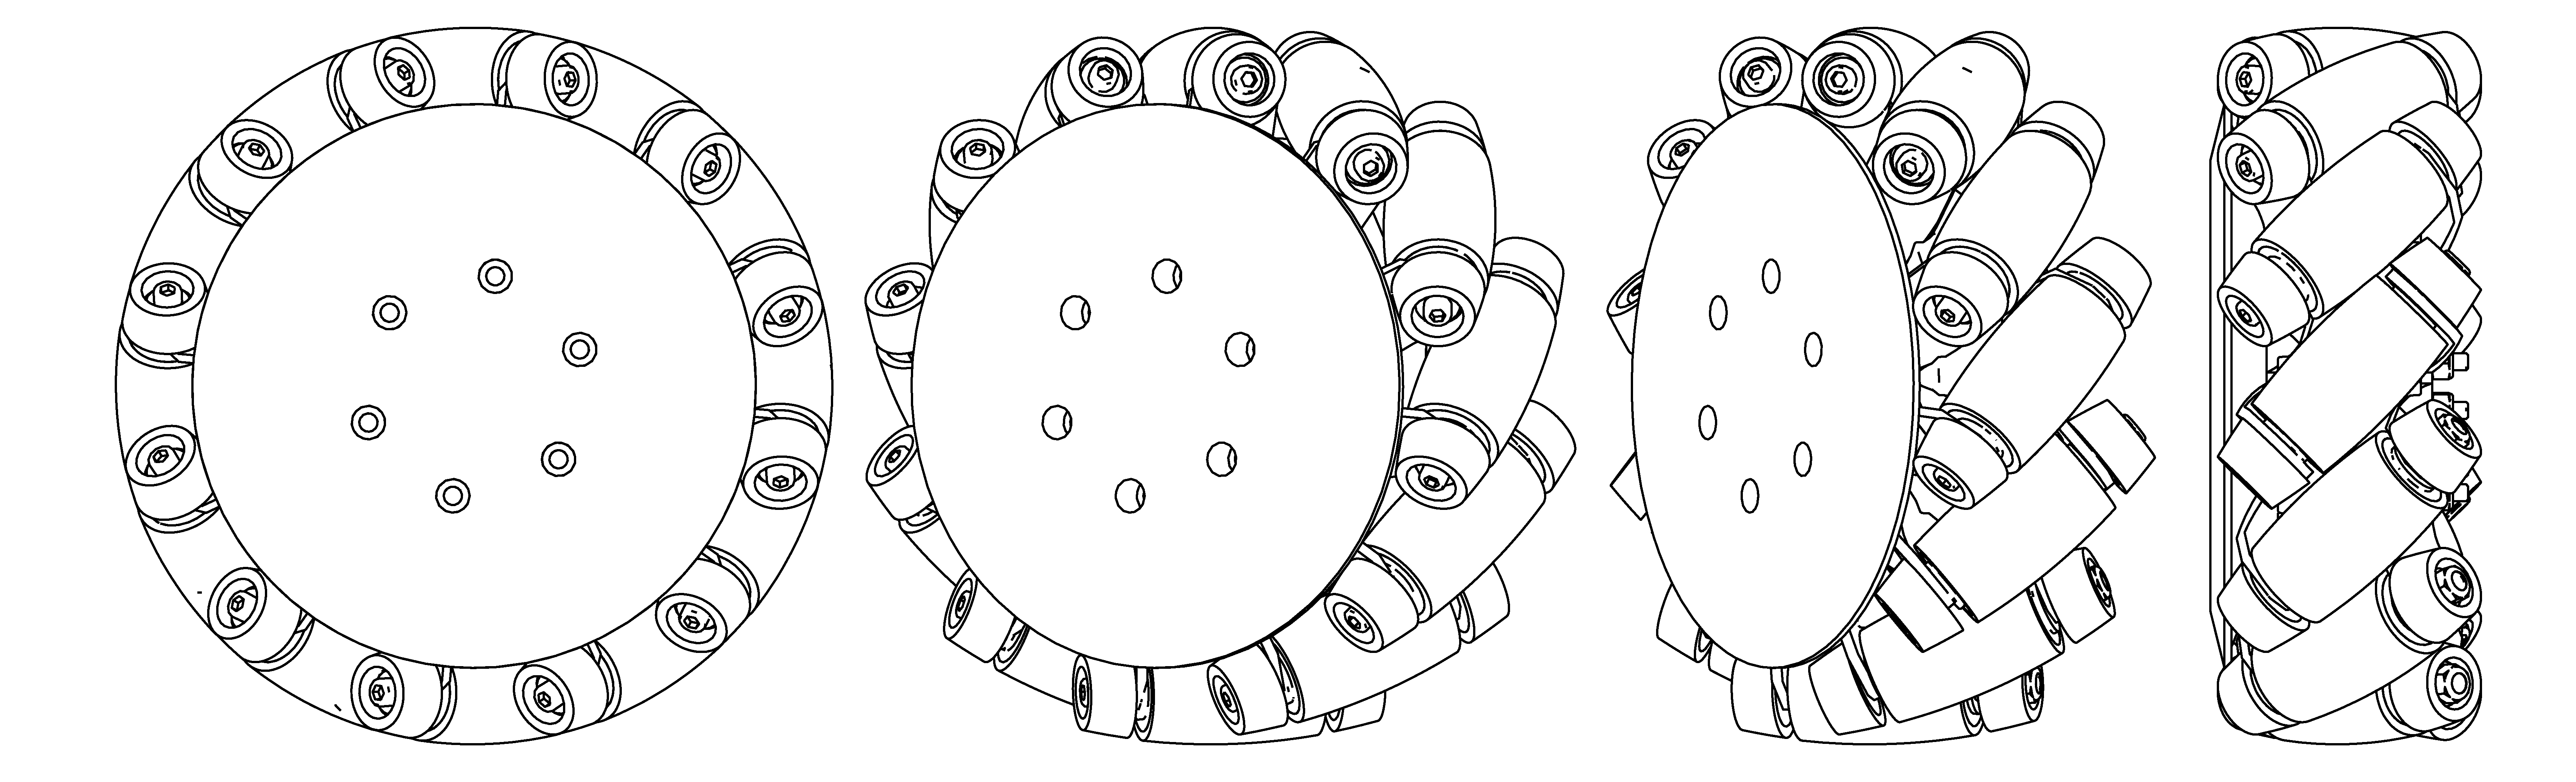
\includegraphics[width=\textwidth]{graphics/wheel.pdf}
		\begin{itemize}
			\item Każde koło ma 12 pasywnych rolek.
			\item Rolka jest obrócona o 45\textdegree{} względem płaszczyzny koła.
			\item Punkt kontaktu powinien płynnie przechodzić z rolki na rolkę.
			\item Koło pod wpływem momentu siły i tarcia podłoża generuje dwa wektory siły, zamiast jednego.
		\end{itemize}
	\end{frame}
	\begin{frame}
		\frametitle{Dodatkowy wektor}
		\centering
		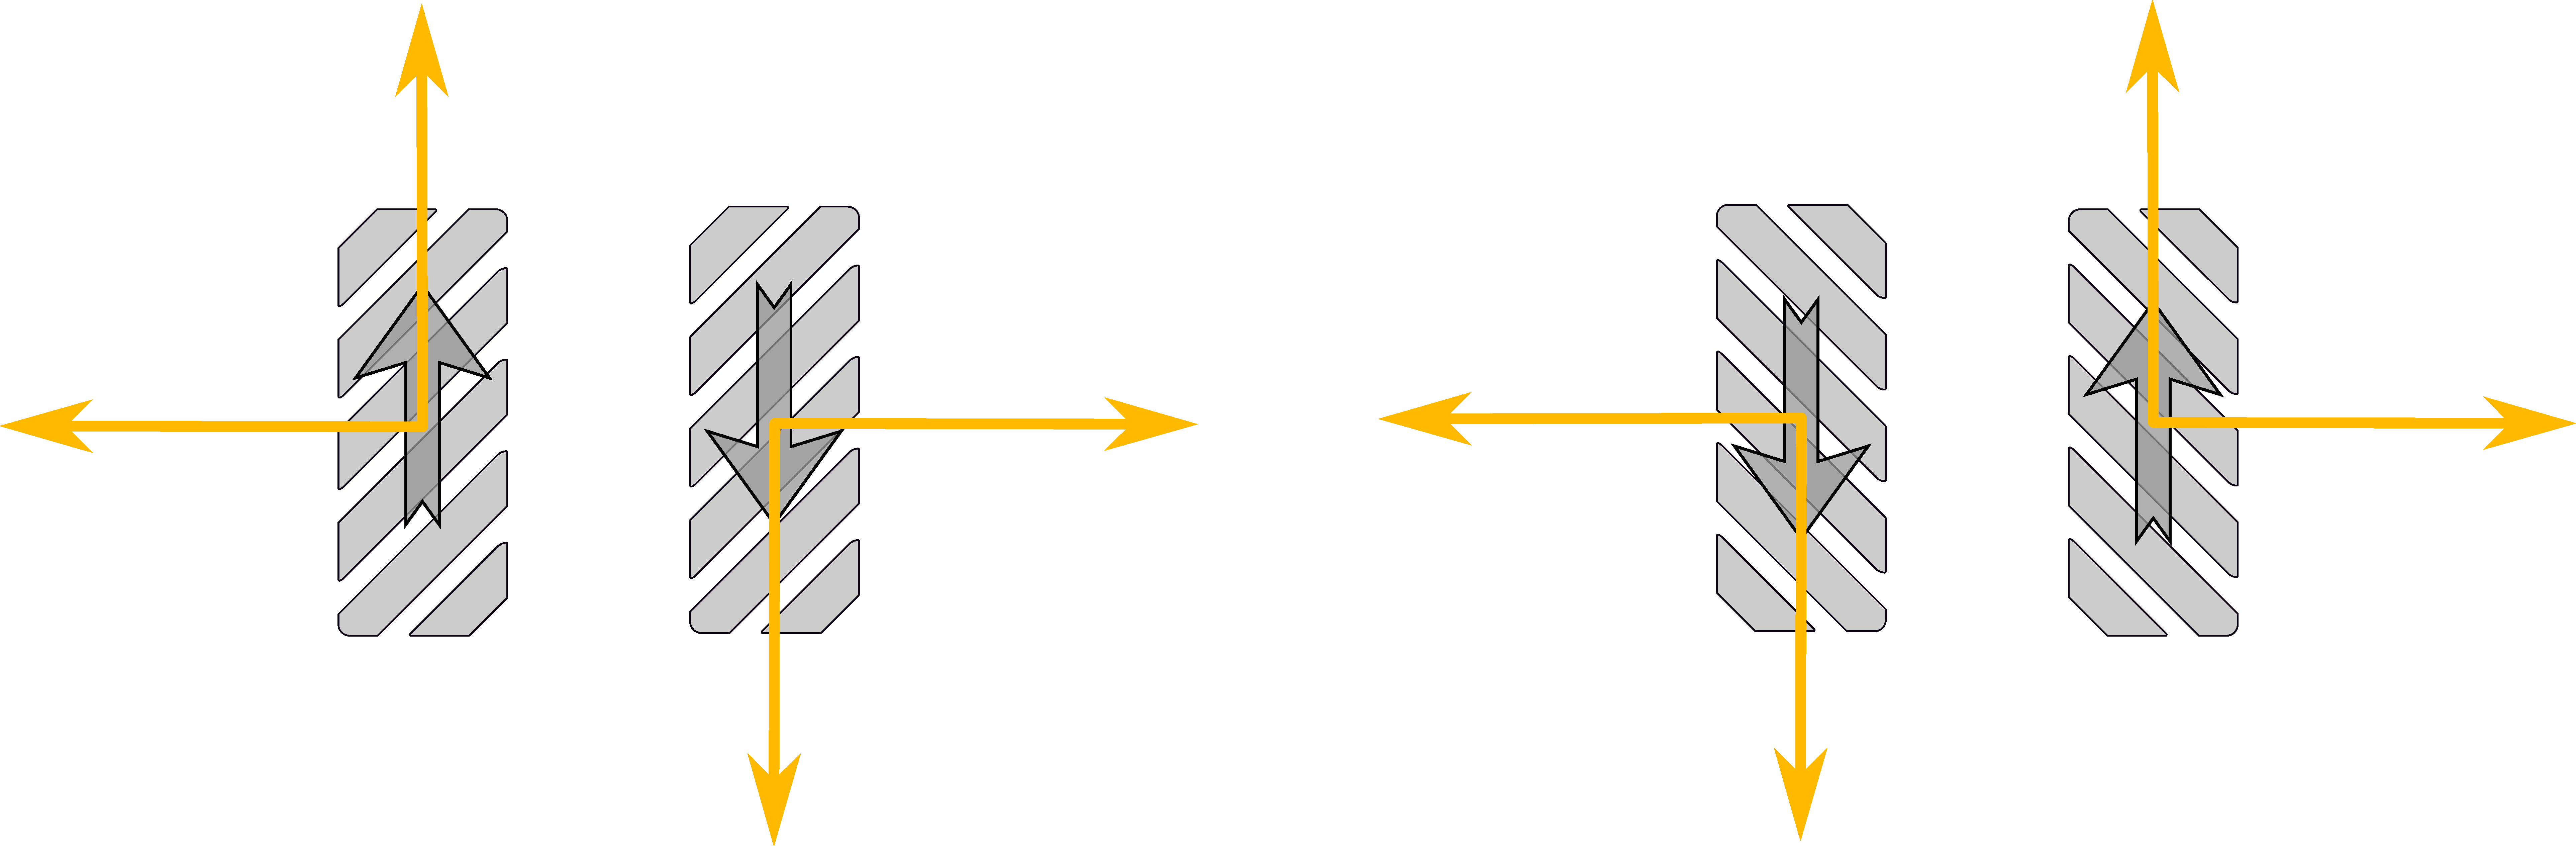
\includegraphics[width=\textwidth]{graphics/vectors.pdf} \\
		Standardowe koło używając tarcia przekształca prędkość kątową na liniową w płaszczyźnie obrotu.
		Specjalne koło Mecanum ma dodatkowy wektor równoległy do osi obrotu, zatem prędkość wypadkowa jest obrócona o 45\textdegree.
	\end{frame}
	\begin{frame}
		\frametitle{Kierunki ruchu}
		\centering
		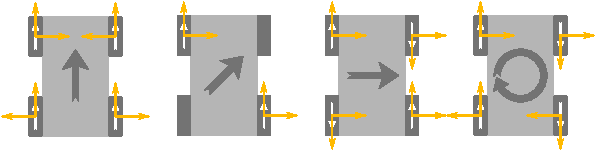
\includegraphics[width=\textwidth]{graphics/dirs.pdf} \\
		Poprzez znoszenie się składowych prędkości, robot może poruszać się w kierunkach nieosiągalnych dla pojazdów o zwykłych kołach.
	\end{frame}
	\begin{frame}
		\frametitle{Kinematyka}
		\[
		\begin{bmatrix}
		v_x \\
		v_y \\
		\omega_z \\
		\end{bmatrix}
		=
		\frac{r}{4}
		\begin{bmatrix}
		-1 & 1 & -1 & 1 \\
		1 & 1 & 1 & 1 \\
		\frac{2}{a+b} & \frac{-2}{a+b} & \frac{-2}{a+b} & \frac{2}{a+b} \\
		\end{bmatrix}
		\begin{bmatrix}
		\omega_1 \\
		\omega_2 \\
		\omega_3 \\
		\omega_4 \\
		\end{bmatrix}
		\]
		\centering
		\includegraphics[width=0.5\textwidth]{graphics/base_dims.pdf} 
	\end{frame}

	\section{Implementacja}
	\begin{frame}
		\frametitle{Modele}
		\begin{columns}[c]
			\column{0.4\textwidth}
			\centering
			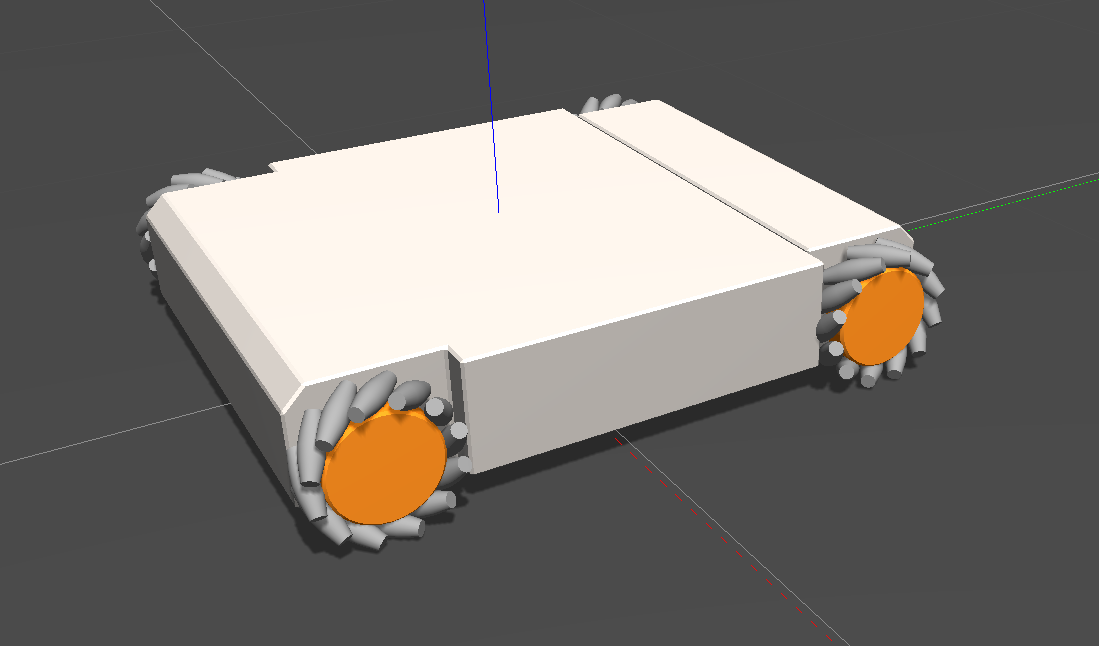
\includegraphics[width=\textwidth]{graphics/model.png} \\
			Dynamiczny model platformy.
			\column{0.6\textwidth}
			Uproszczone modele dynamiki:
			\begin{itemize}
				\item Model dynamiczny w Gazebo.
				\item Model dynamiczny w V-Repie.
			\end{itemize}
			Matematycznie dokładne modele kinematyki:
			\begin{itemize}
				\item Model kinematyki prostej --- koła na prędkość.
				\item Model kinematyki odwrotnej --- prędkość na koła.
			\end{itemize}
		\end{columns}
	\end{frame}
	\begin{frame}
		\frametitle{Struktura projektu}
		\centering
		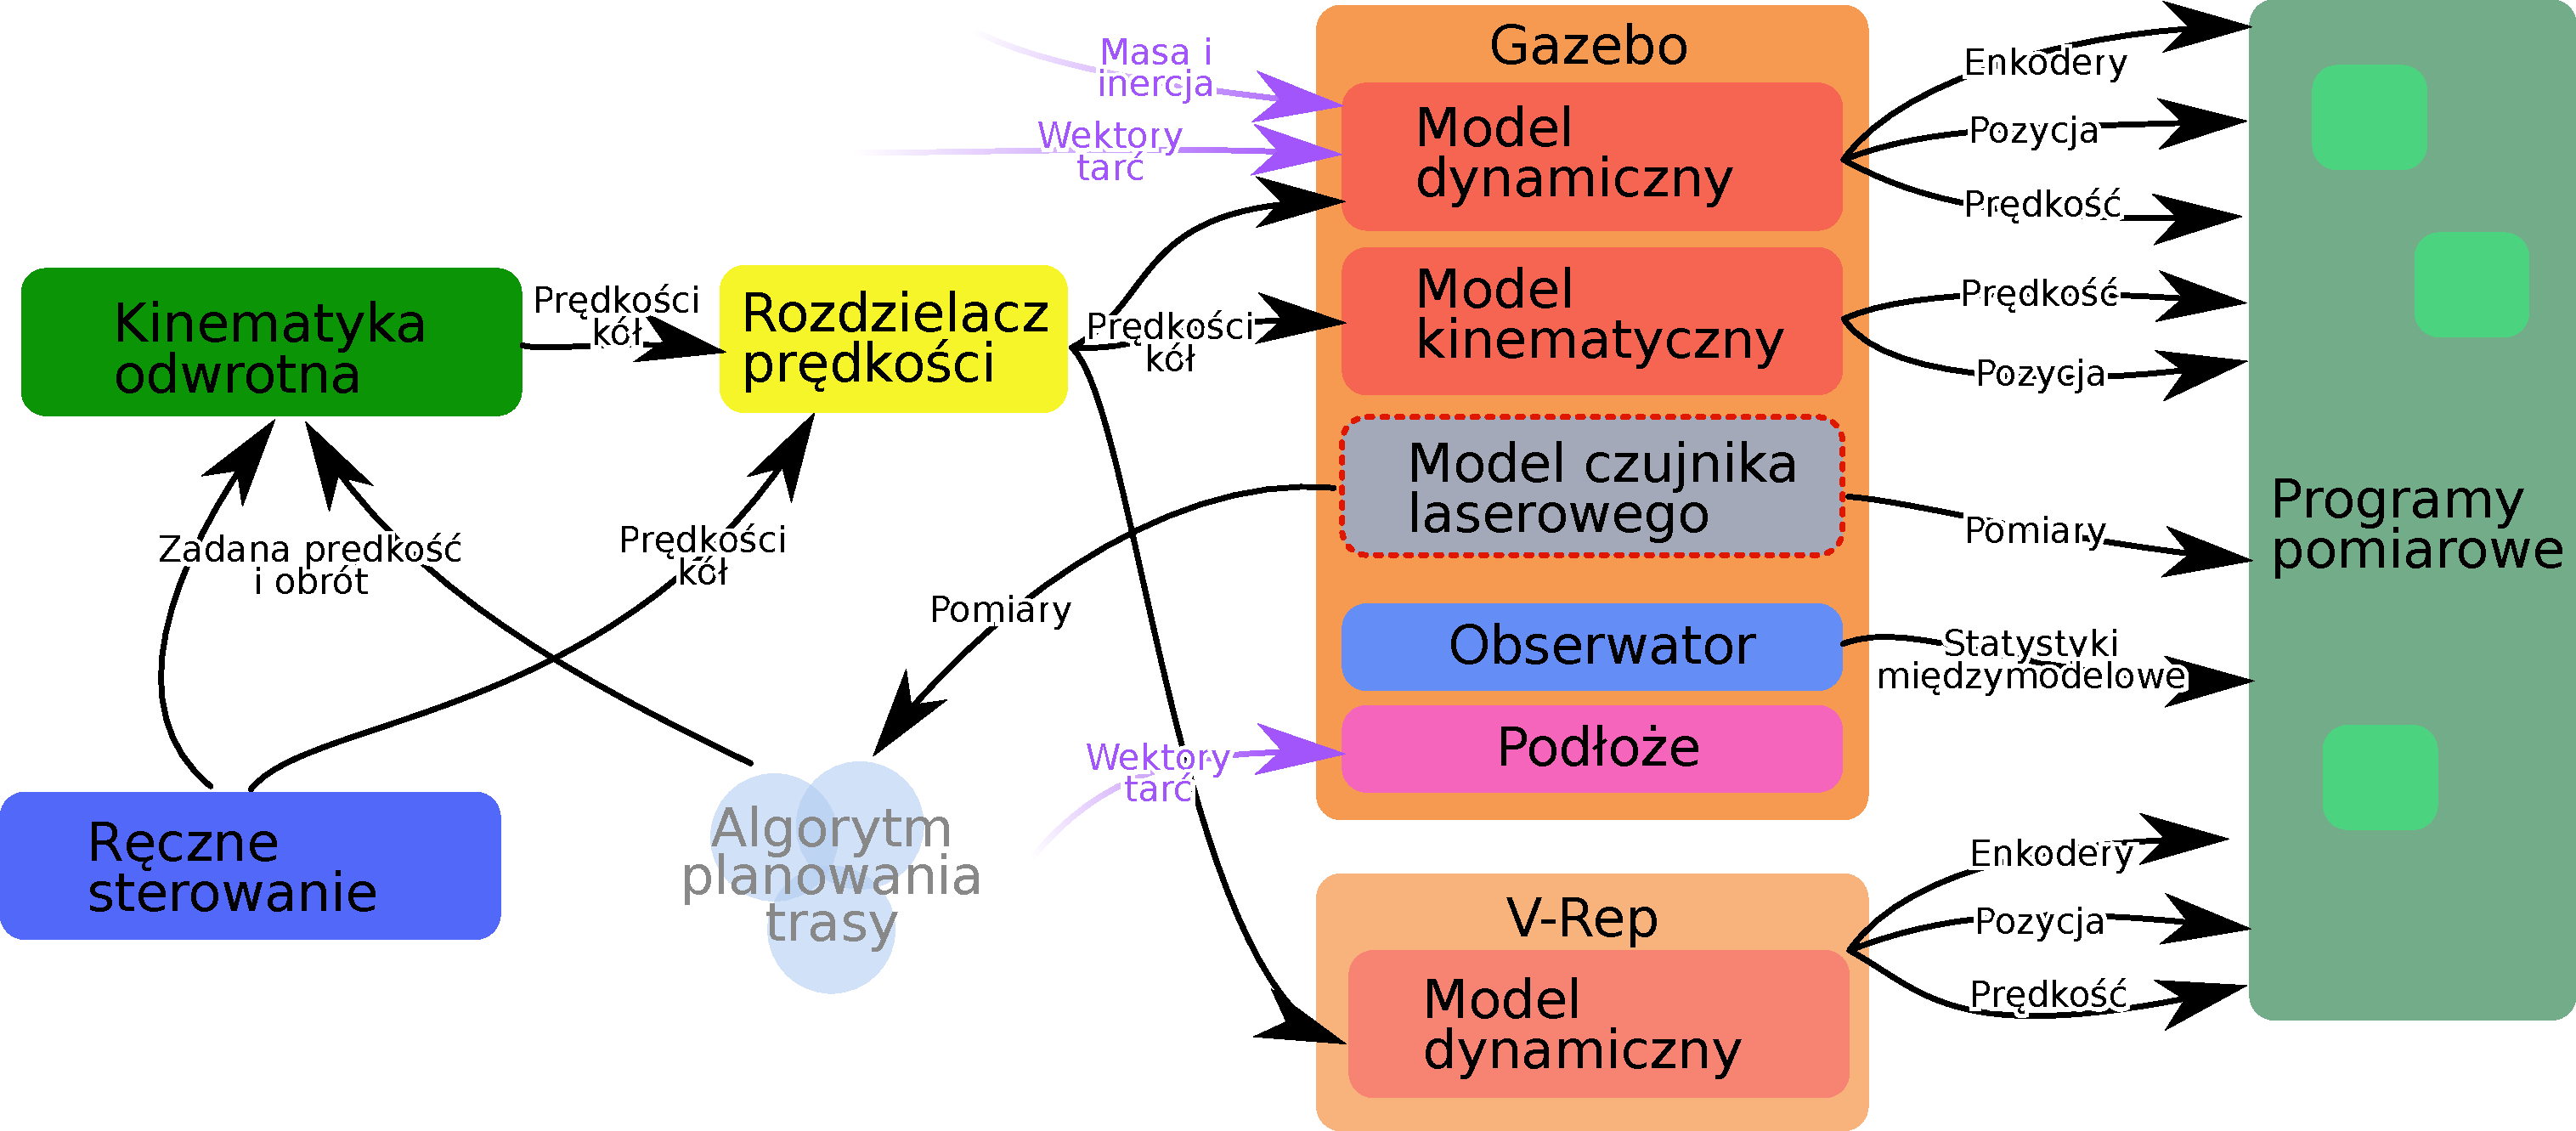
\includegraphics[width=\textwidth]{graphics/comm.pdf} 
	\end{frame}
	\section{Pomiary}
	\begin{frame}
		\frametitle{Sprzęt i wersje programów}
		Eksperymenty przeprowadzono na dobrej jakości sprzęcie i możliwie najaktualniejszych wersjach programów.
		\begin{itemize}
			\item System operacyjny Ubuntu LTS Xenial Xerus
			\item ROS Kinetic Kame
			\item V-Rep 3.4.0
		\end{itemize}
		\begin{itemize}
			\item Intel i7-4720HQ 2.60GHz
			\item 16 GiB RAM
			\item Renderowanie na wbudowanej karcie graficznej
		\end{itemize}
		W czasie testów użycie procesora nigdy nie wyniosło 100\%.
	\end{frame}
	\begin{frame}
		\frametitle{Obszar testów}
		\centering
		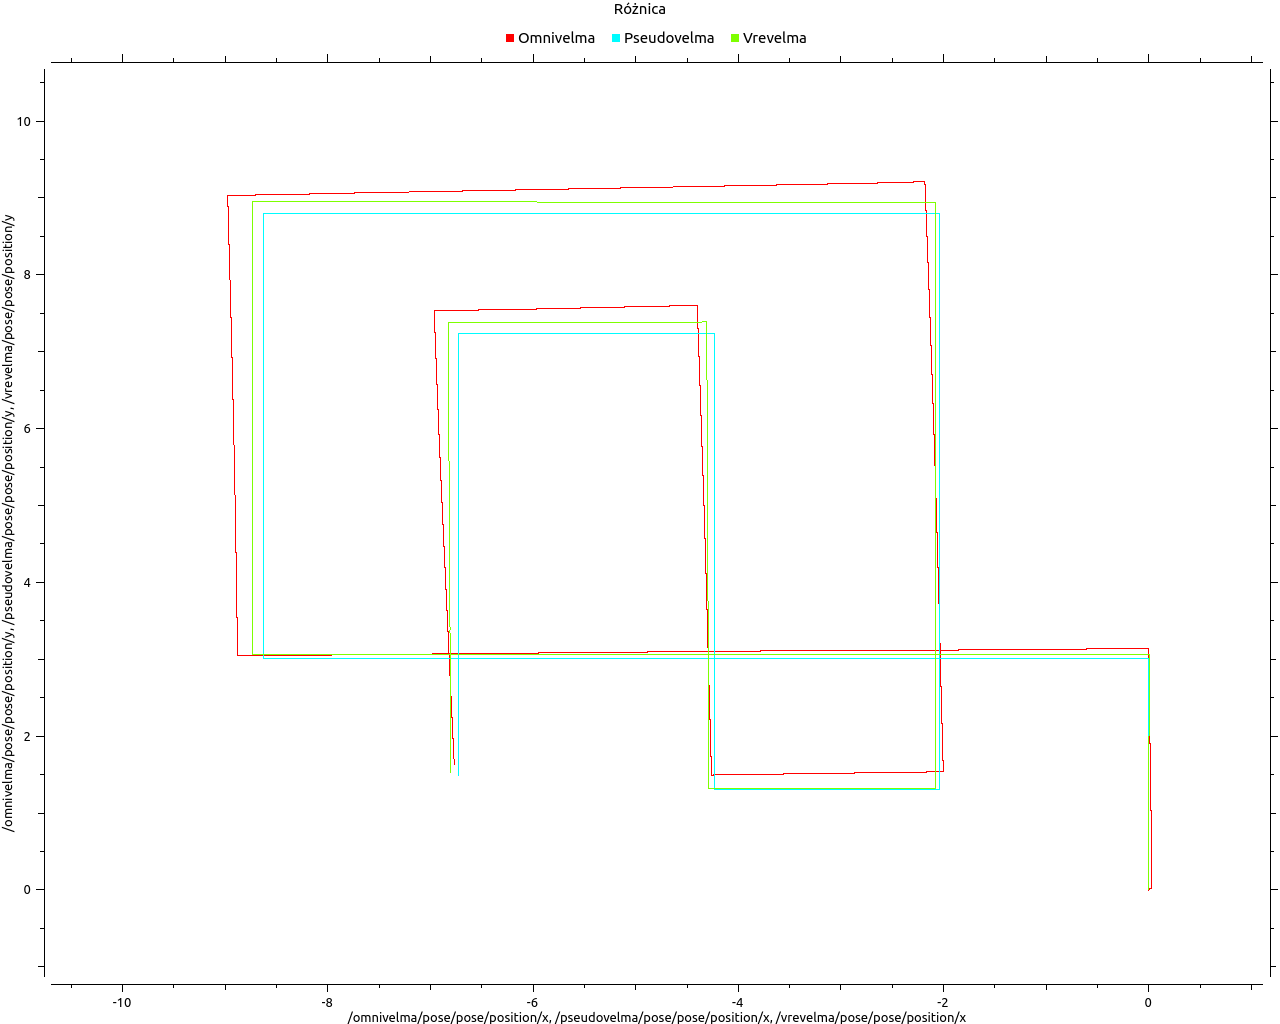
\includegraphics[width=0.8\textwidth]{graphics/track_1.png} \\
		Prosty przebieg bez zmiany orientacji platformy.
	\end{frame}
	\begin{frame}
		\frametitle{Powtarzalność przebiegu}
		\centering
		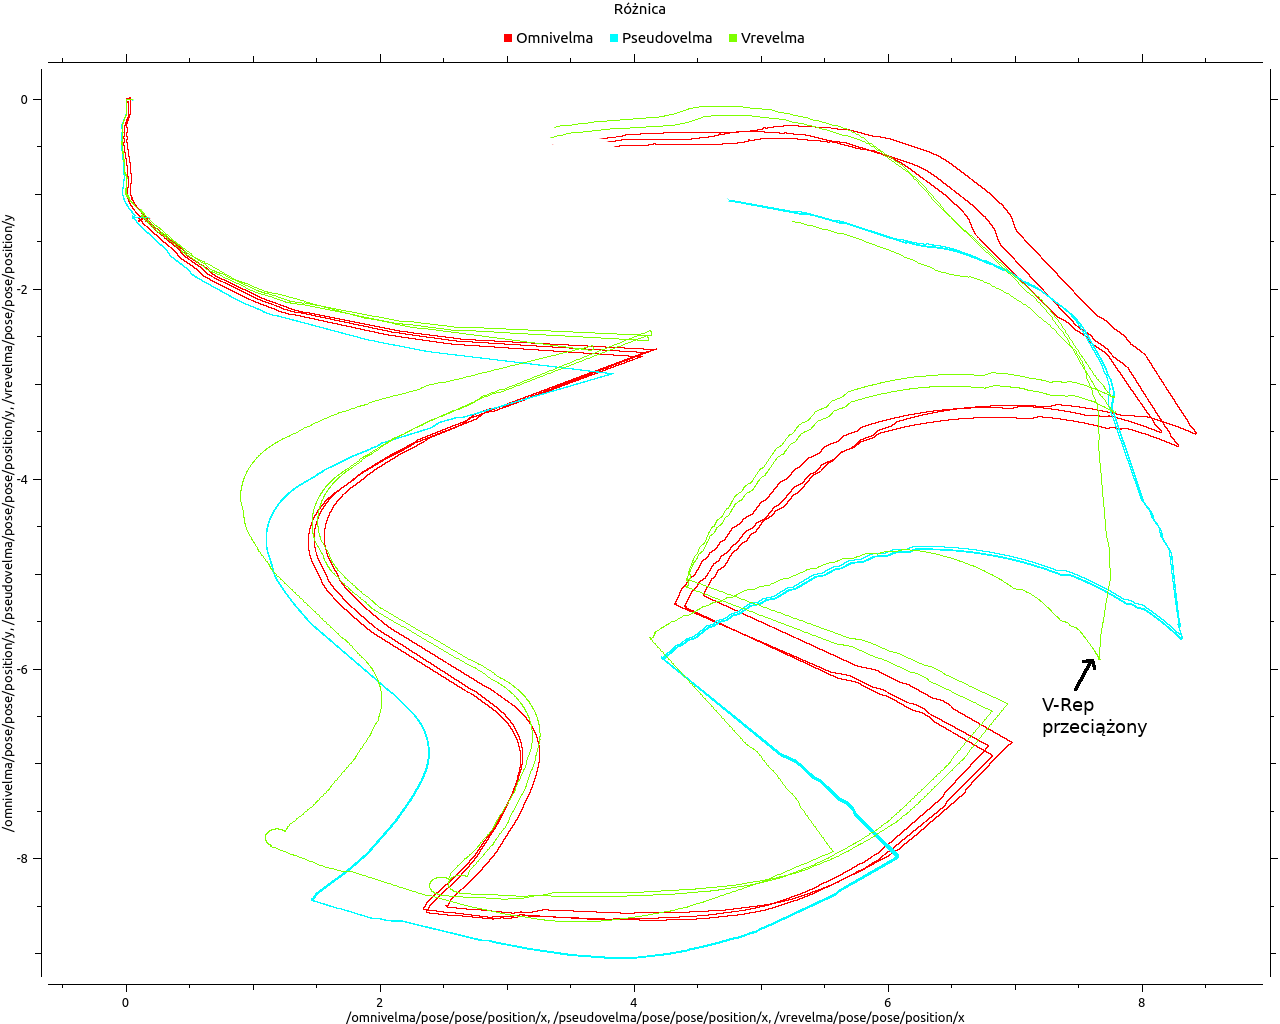
\includegraphics[width=0.8\textwidth]{graphics/bag_3.png} \\
		Robot sterowany binarnymi prędkościami kół.
	\end{frame}
	\begin{frame}
		\frametitle{Badanie odometrii}
		\centering
		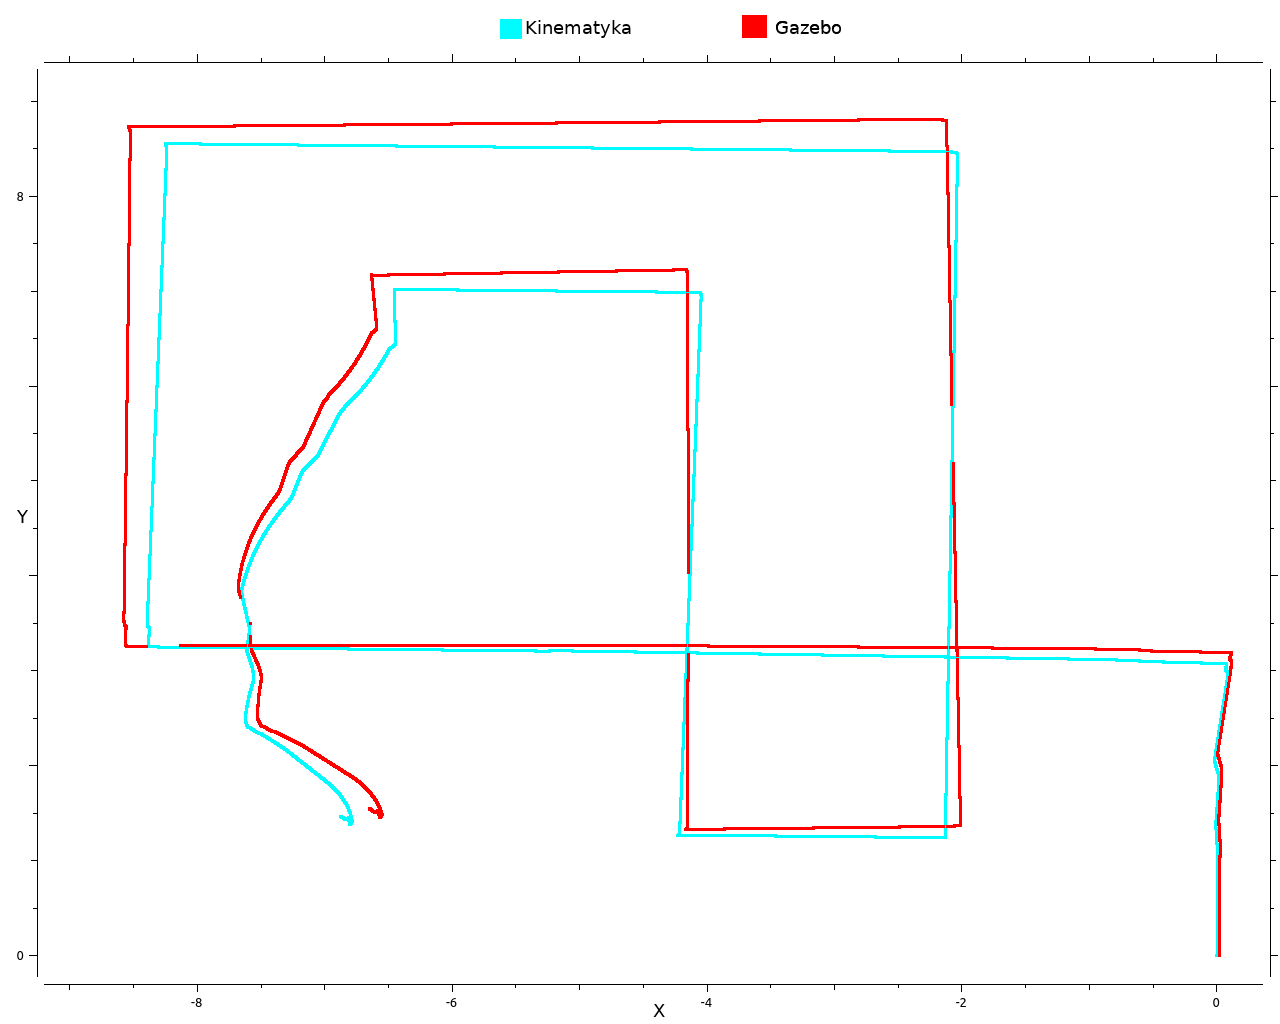
\includegraphics[width=0.7\textwidth]{graphics/reen_1.png} \\
		Model kinematyczny porusza się na podstawie danych generowanych przez enkodery w modelu dynamicznym.
	\end{frame}
	\begin{frame}
		\frametitle{Pokaz?}
		Pokaz na żywo, bądź film.
	\end{frame}
 
	\section{Podsumowanie}
	\begin{frame}
		\frametitle{Podsumowanie}
		\begin{itemize}
			\item Opracowano 3 modele symulacyjne i model pomocniczy, które pozwalają na symulację dynamiki i kinematyki.
			\item Modele mają różną budowę wewnętrzną i działają na różnych symulatorach.
			\item Przebiegi ścieżek są wystarczająco dobrze zbliżone do siebie.
			\item Modele generują dane z zasymulowanych czujników.
			\item Stworzono model podłoża o zmiennym współczynniku tarcia.
			\item Stworzono zestaw programów ułatwiających testowanie.
		\end{itemize}
	\end{frame}
	\begin{frame}
		\frametitle{Perspektywy rozwoju}
		\begin{itemize}
			\item Porównanie działania modeli i robota przy tym samym sterowaniu.
			\item Usprawnienie interfejsu do sterowania ręcznego.
			\item Próba implementacji modelu czujnika laserowego.
			\item Szczegółowa analiza modeli i określenie przyczyn rozbieżności.
			\item Dopracowanie w modelach współczynników takich, jak masy, tarcia i inercja.
		\end{itemize}
	\end{frame}
	\begin{frame}
		\frametitle{Koniec}
		\centering
		Dziękuję za uwagę.\\
		Projekt i ta prezentacja znajdują się na \url{https://github.com/Antyradek/omnivelma}.
	\end{frame}
\end{document}